% Unit inventory (Section S5). Written during the journal revision (agent S,
% 2026-10-13) from the inventory paragraphs of sections/results.tex and the
% status rules of the rule-assembled attempt; the split of the invalid units
% by cause tabulates the released curves (public aggregates, cell at a = 0).
% Round 6: cites the plain-text README uploaded with Online Resource 2.

The prespecified inventory has 46 comparison grids, each crossed with the nine signal shares and the nine strengths of influence: \resultnum{v4.protocol.units.all}{414} units of nine cells each. A unit is one comparison (persistence model, channel and configuration) at one $r$. Its status at the close or release is one of four:
\begin{description}
\item[Complete and valid.] All nine strengths were executed, and the zero-strength cell is available with a band containing 0.5. Gaps at positive strengths censor boundaries but do not invalidate the unit.
\item[Complete but invalid.] All nine strengths were executed, but the zero-strength check failed: the band at $a=0$ excluded 0.5, or the zero-strength cell was a gap. The unit's boundaries are suppressed; its cells stay in the records.
\item[Partial at the operational close.] Some strengths were not executed when the compute window closed.
\item[Not started.] No strength was executed at the close.
\end{description}
These statuses are operational categories of the protocol: ``valid'' records that the zero-strength check passed, not that the unit's intervals have been shown to cover. The main curve is valid only if all nine units of B on the observed channel are complete and valid. The archived machine-readable inventory stores these statuses as Portuguese strings; Table~\ref{tab:glossary-states} maps them to the names used here.

When the results became available, \resultnum{v4.inv.n_valid}{342} of the \resultnum{v4.protocol.units.all}{414} units were complete and valid, \resultnum{v4.inv.n_invalid}{72} were complete but invalid, \resultnum{v4.inv.n_partial}{0} were partial at the operational close and \resultnum{v4.inv.n_not_started}{0} had not started (Table~\ref{tab:v4-T4}, Fig.~\ref{fig:inventory-status}). Every tier therefore finished. By tier: all \resultnum{v4.tab.T4.1-all-all-all.valid}{9} units of the main curve against B were complete and valid, so the main curve is valid under the frozen rule; of the \resultnum{v4.tab.T4.2-all-all-all.units}{36} units of the secondary persistence models, \resultnum{v4.tab.T4.2-all-all-all.valid}{27} were complete and valid and \resultnum{v4.inv.t2.n_invalid}{9} complete but invalid; the measurement-control tier ended with \resultnum{v4.inv.t3.n_valid}{243} of its \resultnum{v4.protocol.units.t3}{270} units complete and valid and \resultnum{v4.inv.t3.n_incomplete}{0} not started or partial; \resultnum{v4.inv.t4.n_valid}{45} of \resultnum{v4.protocol.units.t4}{45} response-channel units and \resultnum{v4.inv.t5.n_valid}{9} of \resultnum{v4.protocol.units.t5}{45} mechanism units were complete and valid; and of the \resultnum{v4.protocol.units.t6}{9} units with \resultnum{v4.protocol.steps}{24} update steps per wave, \resultnum{v4.inv.t6.n_valid}{9} were complete and valid. Only complete units contribute boundaries and AUC profiles.

\paragraph{The 72 invalid units, by cause.}
All \resultnum{j.inventory.invalid.total}{72} complete-but-invalid units fall into two groups, with \resultnum{j.inventory.invalid.other}{0} units outside them.
\begin{itemize}
\item \resultnum{j.inventory.invalid.c_related}{36} units involve persistence model C, whose persistence arm alone receives heteroscedastic error and heaping, so that the two arms differ at zero strength by construction. In the \resultnum{v4.tab.T4.2-C-observed-main.invalid}{9} units of the other-models comparison and the \resultnum{v4.tab.T4.3-C-observed-mobility.invalid}{9} mobility units on the observed channel, the band at $a=0$ excluded 0.5: the zero-strength point AUC against C was \resultnum{j.models.C.zero_auc.min}{1.000} at every share. In \resultnum{v4.tab.T4.3-C-latent-main.invalid}{7} latent-control units, \resultnum{v4.tab.T4.3-C-latent-rank-main.invalid}{4} latent-rank-control units and \resultnum{v4.tab.T4.3-C-latent-mobility.invalid}{7} latent mobility units of C, the zero-strength cell was a gap because the accepted fit failed independent validation in both attempts.
\item \resultnum{j.inventory.invalid.anchoring_sensitivities}{36} units are the anchoring sensitivities, nine for each $\omega\in\{0.25,0.50,0.75,1\}$. With $\omega>0$ the influence arm is pulled toward its initial states at every step, while B has no anchoring, so no identity of the arms at zero strength is claimed; with $\omega=1$ the latent states never change, whatever $a$ is. At $\omega=0.25$ the band at $a=0$ excluded 0.5 in all \resultnum{v4.tab.T4.5-B-observed-omega025.invalid}{9} units. At $\omega=0.50$ the zero-strength cell was a family-limit gap in all \resultnum{v4.tab.T4.5-B-observed-omega050.invalid}{9} units; at $\omega=0.75$ it was a family-limit gap in \resultnum{j.inventory.invalid.omega075.zero_gap.family_limit}{5} units and another solver gap in \resultnum{j.inventory.invalid.omega075.zero_gap.solver}{4}; at $\omega=1$, a family-limit gap in \resultnum{j.inventory.invalid.omega100.zero_gap.family_limit}{2} and another solver gap in \resultnum{j.inventory.invalid.omega100.zero_gap.solver}{7}. These units carry no information about $a$: they check that the anchored arm and B differ at zero strength, which they do by construction.
\end{itemize}

\paragraph{Gap cells.}
The inventory also counts the gap cells of the released curves by kind. In the control units, \resultnum{v4.t3.gap.dependency}{330} cells are dependency gaps because the observed fit they reuse failed or is missing. The two propagation gaps recorded under amendment v4.4 are both in units of D at $r=0.60$ (Section~\ref{sec:record-execution}). Gaps are never counted as AUCs below the target or as evidence that separation is impossible; family limits are gaps, not failures.

\paragraph{Online Resource 2.}
Online Resource~2 (\code{online-resource-2-units.csv}) is the table of all units in English, uploaded with a plain-text README that lists its columns, the scenario legend and the translation of the status labels. It is derived from the released all-units table: it keeps the same rows and columns and translates the Portuguese labels into the names used here, with no other change. The released original, with its Portuguese status labels, stays in the archive. The table gives, for every unit, its tier, persistence model, channel, configuration, $r$, the mark of the share examined during calibration (column \code{exposure}, which keeps the record term calibration-exposed), the main-curve flag (empty in every row, because the main curve is valid), status, zero-strength check (column \code{null_gate}), gap counts by kind, first and sustained boundaries with their intervals, region (with the labels of Table~\ref{tab:glossary-terms}; ``censored (gap)'' is the censored label), the boundaries at the secondary targets 0.60 and 0.80, the band-monotonicity flag, the critical value and whether it exceeded the 2.7729 floor.

% Generated by ic_study.analysis.v4_report_export from the v4 report with
% manifest SHA-256 6608b3960eb73011caca97870a4ffd3dbfbcd4c2df09bbbcb576c1c9452cf981.
% Edited during the journal revision (agent S, 2026-10-13): captions, headers and
% categorical cells in plain English; every number keeps its \resultnum binding.
\begin{table*}[tp]
\caption{Inventory at the close: units by status for each prespecified configuration, for each tier and in total, and the gap cells of the released curves by kind. Tiers: 1 main curve against B; 2 secondary persistence models; 3 measurement controls (latent, ordinal with $r=1$, latent rank) and mobility summaries; 4 response-channel sensitivities (persistent response style, $c=0.25$ or 0.50; panel conditioning, $\delta=0.10$ or 0.20; response style and conditioning, $c=0.50$, $\delta=0.20$, exploratory); 5 mechanism sensitivities (attraction only, $b=0$; anchoring; complete anchoring, $\omega=1$); 6 24 update steps per wave (Table~\ref{tab:glossary-gate}). Status: NS not started, P partial at the operational close, CI complete but invalid, CV complete and valid (Section~\ref{sec:inventory}; the archive's machine-readable records store these four statuses in Portuguese). Gap cells: scr.\ family limit at the feasibility screen, with no solver evaluation; fam.\ family limit on the profile; sol.\ other solver status; val.\ accepted fit that failed validation in both attempts; dep.\ control whose observed fit failed or is missing; prop.\ ill-conditioned nuisance propagation recorded as a gap under amendment v4.4 (Section~\ref{sec:record-execution}). Family limits are gaps, not failures.}\label{tab:v4-T4}
\centering\scriptsize
\setlength{\tabcolsep}{1.5pt}
\begin{tabular}{lllp{2.3cm}rrrrrrrrrrr}
\toprule
Tier & Model & Channel & Configuration & Units & NS & P & CI & CV & scr. & fam. & sol. & val. & dep. & prop. \\
\midrule
\resultnum{v4.tab.T4.1-B-observed-main.tier}{1} & B & observed & main & \resultnum{v4.tab.T4.1-B-observed-main.units}{9} & \resultnum{v4.tab.T4.1-B-observed-main.not_started}{0} & \resultnum{v4.tab.T4.1-B-observed-main.partial}{0} & \resultnum{v4.tab.T4.1-B-observed-main.invalid}{0} & \resultnum{v4.tab.T4.1-B-observed-main.valid}{9} & \resultnum{v4.tab.T4.1-B-observed-main.gaps_screened}{0} & \resultnum{v4.tab.T4.1-B-observed-main.gaps_family_limit}{0} & \resultnum{v4.tab.T4.1-B-observed-main.gaps_solver}{3} & \resultnum{v4.tab.T4.1-B-observed-main.gaps_validation}{0} & \resultnum{v4.tab.T4.1-B-observed-main.gaps_dependency}{0} & \resultnum{v4.tab.T4.1-B-observed-main.gaps_propagation}{0} \\
\resultnum{v4.tab.T4.2-A-observed-main.tier}{2} & A & observed & main & \resultnum{v4.tab.T4.2-A-observed-main.units}{9} & \resultnum{v4.tab.T4.2-A-observed-main.not_started}{0} & \resultnum{v4.tab.T4.2-A-observed-main.partial}{0} & \resultnum{v4.tab.T4.2-A-observed-main.invalid}{0} & \resultnum{v4.tab.T4.2-A-observed-main.valid}{9} & \resultnum{v4.tab.T4.2-A-observed-main.gaps_screened}{0} & \resultnum{v4.tab.T4.2-A-observed-main.gaps_family_limit}{0} & \resultnum{v4.tab.T4.2-A-observed-main.gaps_solver}{0} & \resultnum{v4.tab.T4.2-A-observed-main.gaps_validation}{0} & \resultnum{v4.tab.T4.2-A-observed-main.gaps_dependency}{0} & \resultnum{v4.tab.T4.2-A-observed-main.gaps_propagation}{0} \\
\resultnum{v4.tab.T4.2-C-observed-main.tier}{2} & C & observed & main & \resultnum{v4.tab.T4.2-C-observed-main.units}{9} & \resultnum{v4.tab.T4.2-C-observed-main.not_started}{0} & \resultnum{v4.tab.T4.2-C-observed-main.partial}{0} & \resultnum{v4.tab.T4.2-C-observed-main.invalid}{9} & \resultnum{v4.tab.T4.2-C-observed-main.valid}{0} & \resultnum{v4.tab.T4.2-C-observed-main.gaps_screened}{0} & \resultnum{v4.tab.T4.2-C-observed-main.gaps_family_limit}{0} & \resultnum{v4.tab.T4.2-C-observed-main.gaps_solver}{22} & \resultnum{v4.tab.T4.2-C-observed-main.gaps_validation}{0} & \resultnum{v4.tab.T4.2-C-observed-main.gaps_dependency}{0} & \resultnum{v4.tab.T4.2-C-observed-main.gaps_propagation}{0} \\
\resultnum{v4.tab.T4.2-D-observed-main.tier}{2} & D & observed & main & \resultnum{v4.tab.T4.2-D-observed-main.units}{9} & \resultnum{v4.tab.T4.2-D-observed-main.not_started}{0} & \resultnum{v4.tab.T4.2-D-observed-main.partial}{0} & \resultnum{v4.tab.T4.2-D-observed-main.invalid}{0} & \resultnum{v4.tab.T4.2-D-observed-main.valid}{9} & \resultnum{v4.tab.T4.2-D-observed-main.gaps_screened}{0} & \resultnum{v4.tab.T4.2-D-observed-main.gaps_family_limit}{33} & \resultnum{v4.tab.T4.2-D-observed-main.gaps_solver}{4} & \resultnum{v4.tab.T4.2-D-observed-main.gaps_validation}{0} & \resultnum{v4.tab.T4.2-D-observed-main.gaps_dependency}{0} & \resultnum{v4.tab.T4.2-D-observed-main.gaps_propagation}{1} \\
\resultnum{v4.tab.T4.2-E-observed-main.tier}{2} & E & observed & main & \resultnum{v4.tab.T4.2-E-observed-main.units}{9} & \resultnum{v4.tab.T4.2-E-observed-main.not_started}{0} & \resultnum{v4.tab.T4.2-E-observed-main.partial}{0} & \resultnum{v4.tab.T4.2-E-observed-main.invalid}{0} & \resultnum{v4.tab.T4.2-E-observed-main.valid}{9} & \resultnum{v4.tab.T4.2-E-observed-main.gaps_screened}{0} & \resultnum{v4.tab.T4.2-E-observed-main.gaps_family_limit}{0} & \resultnum{v4.tab.T4.2-E-observed-main.gaps_solver}{3} & \resultnum{v4.tab.T4.2-E-observed-main.gaps_validation}{0} & \resultnum{v4.tab.T4.2-E-observed-main.gaps_dependency}{0} & \resultnum{v4.tab.T4.2-E-observed-main.gaps_propagation}{0} \\
\resultnum{v4.tab.T4.3-A-latent-main.tier}{3} & A & latent & main & \resultnum{v4.tab.T4.3-A-latent-main.units}{9} & \resultnum{v4.tab.T4.3-A-latent-main.not_started}{0} & \resultnum{v4.tab.T4.3-A-latent-main.partial}{0} & \resultnum{v4.tab.T4.3-A-latent-main.invalid}{0} & \resultnum{v4.tab.T4.3-A-latent-main.valid}{9} & \resultnum{v4.tab.T4.3-A-latent-main.gaps_screened}{0} & \resultnum{v4.tab.T4.3-A-latent-main.gaps_family_limit}{0} & \resultnum{v4.tab.T4.3-A-latent-main.gaps_solver}{0} & \resultnum{v4.tab.T4.3-A-latent-main.gaps_validation}{0} & \resultnum{v4.tab.T4.3-A-latent-main.gaps_dependency}{0} & \resultnum{v4.tab.T4.3-A-latent-main.gaps_propagation}{0} \\
\resultnum{v4.tab.T4.3-A-ordinal-one-main.tier}{3} & A & ordinal, $r=1$ & main & \resultnum{v4.tab.T4.3-A-ordinal-one-main.units}{9} & \resultnum{v4.tab.T4.3-A-ordinal-one-main.not_started}{0} & \resultnum{v4.tab.T4.3-A-ordinal-one-main.partial}{0} & \resultnum{v4.tab.T4.3-A-ordinal-one-main.invalid}{0} & \resultnum{v4.tab.T4.3-A-ordinal-one-main.valid}{9} & \resultnum{v4.tab.T4.3-A-ordinal-one-main.gaps_screened}{0} & \resultnum{v4.tab.T4.3-A-ordinal-one-main.gaps_family_limit}{0} & \resultnum{v4.tab.T4.3-A-ordinal-one-main.gaps_solver}{0} & \resultnum{v4.tab.T4.3-A-ordinal-one-main.gaps_validation}{0} & \resultnum{v4.tab.T4.3-A-ordinal-one-main.gaps_dependency}{0} & \resultnum{v4.tab.T4.3-A-ordinal-one-main.gaps_propagation}{0} \\
\resultnum{v4.tab.T4.3-A-latent-rank-main.tier}{3} & A & latent rank & main & \resultnum{v4.tab.T4.3-A-latent-rank-main.units}{9} & \resultnum{v4.tab.T4.3-A-latent-rank-main.not_started}{0} & \resultnum{v4.tab.T4.3-A-latent-rank-main.partial}{0} & \resultnum{v4.tab.T4.3-A-latent-rank-main.invalid}{0} & \resultnum{v4.tab.T4.3-A-latent-rank-main.valid}{9} & \resultnum{v4.tab.T4.3-A-latent-rank-main.gaps_screened}{0} & \resultnum{v4.tab.T4.3-A-latent-rank-main.gaps_family_limit}{0} & \resultnum{v4.tab.T4.3-A-latent-rank-main.gaps_solver}{0} & \resultnum{v4.tab.T4.3-A-latent-rank-main.gaps_validation}{0} & \resultnum{v4.tab.T4.3-A-latent-rank-main.gaps_dependency}{0} & \resultnum{v4.tab.T4.3-A-latent-rank-main.gaps_propagation}{0} \\
\resultnum{v4.tab.T4.3-B-latent-main.tier}{3} & B & latent & main & \resultnum{v4.tab.T4.3-B-latent-main.units}{9} & \resultnum{v4.tab.T4.3-B-latent-main.not_started}{0} & \resultnum{v4.tab.T4.3-B-latent-main.partial}{0} & \resultnum{v4.tab.T4.3-B-latent-main.invalid}{0} & \resultnum{v4.tab.T4.3-B-latent-main.valid}{9} & \resultnum{v4.tab.T4.3-B-latent-main.gaps_screened}{0} & \resultnum{v4.tab.T4.3-B-latent-main.gaps_family_limit}{0} & \resultnum{v4.tab.T4.3-B-latent-main.gaps_solver}{0} & \resultnum{v4.tab.T4.3-B-latent-main.gaps_validation}{0} & \resultnum{v4.tab.T4.3-B-latent-main.gaps_dependency}{3} & \resultnum{v4.tab.T4.3-B-latent-main.gaps_propagation}{0} \\
\resultnum{v4.tab.T4.3-B-ordinal-one-main.tier}{3} & B & ordinal, $r=1$ & main & \resultnum{v4.tab.T4.3-B-ordinal-one-main.units}{9} & \resultnum{v4.tab.T4.3-B-ordinal-one-main.not_started}{0} & \resultnum{v4.tab.T4.3-B-ordinal-one-main.partial}{0} & \resultnum{v4.tab.T4.3-B-ordinal-one-main.invalid}{0} & \resultnum{v4.tab.T4.3-B-ordinal-one-main.valid}{9} & \resultnum{v4.tab.T4.3-B-ordinal-one-main.gaps_screened}{0} & \resultnum{v4.tab.T4.3-B-ordinal-one-main.gaps_family_limit}{0} & \resultnum{v4.tab.T4.3-B-ordinal-one-main.gaps_solver}{0} & \resultnum{v4.tab.T4.3-B-ordinal-one-main.gaps_validation}{0} & \resultnum{v4.tab.T4.3-B-ordinal-one-main.gaps_dependency}{3} & \resultnum{v4.tab.T4.3-B-ordinal-one-main.gaps_propagation}{0} \\
\resultnum{v4.tab.T4.3-B-latent-rank-main.tier}{3} & B & latent rank & main & \resultnum{v4.tab.T4.3-B-latent-rank-main.units}{9} & \resultnum{v4.tab.T4.3-B-latent-rank-main.not_started}{0} & \resultnum{v4.tab.T4.3-B-latent-rank-main.partial}{0} & \resultnum{v4.tab.T4.3-B-latent-rank-main.invalid}{0} & \resultnum{v4.tab.T4.3-B-latent-rank-main.valid}{9} & \resultnum{v4.tab.T4.3-B-latent-rank-main.gaps_screened}{0} & \resultnum{v4.tab.T4.3-B-latent-rank-main.gaps_family_limit}{0} & \resultnum{v4.tab.T4.3-B-latent-rank-main.gaps_solver}{0} & \resultnum{v4.tab.T4.3-B-latent-rank-main.gaps_validation}{0} & \resultnum{v4.tab.T4.3-B-latent-rank-main.gaps_dependency}{3} & \resultnum{v4.tab.T4.3-B-latent-rank-main.gaps_propagation}{0} \\
\resultnum{v4.tab.T4.3-C-latent-main.tier}{3} & C & latent & main & \resultnum{v4.tab.T4.3-C-latent-main.units}{9} & \resultnum{v4.tab.T4.3-C-latent-main.not_started}{0} & \resultnum{v4.tab.T4.3-C-latent-main.partial}{0} & \resultnum{v4.tab.T4.3-C-latent-main.invalid}{7} & \resultnum{v4.tab.T4.3-C-latent-main.valid}{2} & \resultnum{v4.tab.T4.3-C-latent-main.gaps_screened}{0} & \resultnum{v4.tab.T4.3-C-latent-main.gaps_family_limit}{0} & \resultnum{v4.tab.T4.3-C-latent-main.gaps_solver}{0} & \resultnum{v4.tab.T4.3-C-latent-main.gaps_validation}{7} & \resultnum{v4.tab.T4.3-C-latent-main.gaps_dependency}{22} & \resultnum{v4.tab.T4.3-C-latent-main.gaps_propagation}{0} \\
\resultnum{v4.tab.T4.3-C-ordinal-one-main.tier}{3} & C & ordinal, $r=1$ & main & \resultnum{v4.tab.T4.3-C-ordinal-one-main.units}{9} & \resultnum{v4.tab.T4.3-C-ordinal-one-main.not_started}{0} & \resultnum{v4.tab.T4.3-C-ordinal-one-main.partial}{0} & \resultnum{v4.tab.T4.3-C-ordinal-one-main.invalid}{0} & \resultnum{v4.tab.T4.3-C-ordinal-one-main.valid}{9} & \resultnum{v4.tab.T4.3-C-ordinal-one-main.gaps_screened}{0} & \resultnum{v4.tab.T4.3-C-ordinal-one-main.gaps_family_limit}{0} & \resultnum{v4.tab.T4.3-C-ordinal-one-main.gaps_solver}{0} & \resultnum{v4.tab.T4.3-C-ordinal-one-main.gaps_validation}{0} & \resultnum{v4.tab.T4.3-C-ordinal-one-main.gaps_dependency}{22} & \resultnum{v4.tab.T4.3-C-ordinal-one-main.gaps_propagation}{0} \\
\resultnum{v4.tab.T4.3-C-latent-rank-main.tier}{3} & C & latent rank & main & \resultnum{v4.tab.T4.3-C-latent-rank-main.units}{9} & \resultnum{v4.tab.T4.3-C-latent-rank-main.not_started}{0} & \resultnum{v4.tab.T4.3-C-latent-rank-main.partial}{0} & \resultnum{v4.tab.T4.3-C-latent-rank-main.invalid}{4} & \resultnum{v4.tab.T4.3-C-latent-rank-main.valid}{5} & \resultnum{v4.tab.T4.3-C-latent-rank-main.gaps_screened}{0} & \resultnum{v4.tab.T4.3-C-latent-rank-main.gaps_family_limit}{0} & \resultnum{v4.tab.T4.3-C-latent-rank-main.gaps_solver}{0} & \resultnum{v4.tab.T4.3-C-latent-rank-main.gaps_validation}{4} & \resultnum{v4.tab.T4.3-C-latent-rank-main.gaps_dependency}{22} & \resultnum{v4.tab.T4.3-C-latent-rank-main.gaps_propagation}{0} \\
\resultnum{v4.tab.T4.3-D-latent-main.tier}{3} & D & latent & main & \resultnum{v4.tab.T4.3-D-latent-main.units}{9} & \resultnum{v4.tab.T4.3-D-latent-main.not_started}{0} & \resultnum{v4.tab.T4.3-D-latent-main.partial}{0} & \resultnum{v4.tab.T4.3-D-latent-main.invalid}{0} & \resultnum{v4.tab.T4.3-D-latent-main.valid}{9} & \resultnum{v4.tab.T4.3-D-latent-main.gaps_screened}{0} & \resultnum{v4.tab.T4.3-D-latent-main.gaps_family_limit}{0} & \resultnum{v4.tab.T4.3-D-latent-main.gaps_solver}{0} & \resultnum{v4.tab.T4.3-D-latent-main.gaps_validation}{0} & \resultnum{v4.tab.T4.3-D-latent-main.gaps_dependency}{38} & \resultnum{v4.tab.T4.3-D-latent-main.gaps_propagation}{0} \\
\resultnum{v4.tab.T4.3-D-ordinal-one-main.tier}{3} & D & ordinal, $r=1$ & main & \resultnum{v4.tab.T4.3-D-ordinal-one-main.units}{9} & \resultnum{v4.tab.T4.3-D-ordinal-one-main.not_started}{0} & \resultnum{v4.tab.T4.3-D-ordinal-one-main.partial}{0} & \resultnum{v4.tab.T4.3-D-ordinal-one-main.invalid}{0} & \resultnum{v4.tab.T4.3-D-ordinal-one-main.valid}{9} & \resultnum{v4.tab.T4.3-D-ordinal-one-main.gaps_screened}{0} & \resultnum{v4.tab.T4.3-D-ordinal-one-main.gaps_family_limit}{0} & \resultnum{v4.tab.T4.3-D-ordinal-one-main.gaps_solver}{0} & \resultnum{v4.tab.T4.3-D-ordinal-one-main.gaps_validation}{0} & \resultnum{v4.tab.T4.3-D-ordinal-one-main.gaps_dependency}{38} & \resultnum{v4.tab.T4.3-D-ordinal-one-main.gaps_propagation}{0} \\
\resultnum{v4.tab.T4.3-D-latent-rank-main.tier}{3} & D & latent rank & main & \resultnum{v4.tab.T4.3-D-latent-rank-main.units}{9} & \resultnum{v4.tab.T4.3-D-latent-rank-main.not_started}{0} & \resultnum{v4.tab.T4.3-D-latent-rank-main.partial}{0} & \resultnum{v4.tab.T4.3-D-latent-rank-main.invalid}{0} & \resultnum{v4.tab.T4.3-D-latent-rank-main.valid}{9} & \resultnum{v4.tab.T4.3-D-latent-rank-main.gaps_screened}{0} & \resultnum{v4.tab.T4.3-D-latent-rank-main.gaps_family_limit}{0} & \resultnum{v4.tab.T4.3-D-latent-rank-main.gaps_solver}{0} & \resultnum{v4.tab.T4.3-D-latent-rank-main.gaps_validation}{0} & \resultnum{v4.tab.T4.3-D-latent-rank-main.gaps_dependency}{38} & \resultnum{v4.tab.T4.3-D-latent-rank-main.gaps_propagation}{0} \\
\resultnum{v4.tab.T4.3-E-latent-main.tier}{3} & E & latent & main & \resultnum{v4.tab.T4.3-E-latent-main.units}{9} & \resultnum{v4.tab.T4.3-E-latent-main.not_started}{0} & \resultnum{v4.tab.T4.3-E-latent-main.partial}{0} & \resultnum{v4.tab.T4.3-E-latent-main.invalid}{0} & \resultnum{v4.tab.T4.3-E-latent-main.valid}{9} & \resultnum{v4.tab.T4.3-E-latent-main.gaps_screened}{0} & \resultnum{v4.tab.T4.3-E-latent-main.gaps_family_limit}{0} & \resultnum{v4.tab.T4.3-E-latent-main.gaps_solver}{0} & \resultnum{v4.tab.T4.3-E-latent-main.gaps_validation}{0} & \resultnum{v4.tab.T4.3-E-latent-main.gaps_dependency}{3} & \resultnum{v4.tab.T4.3-E-latent-main.gaps_propagation}{0} \\
\resultnum{v4.tab.T4.3-E-ordinal-one-main.tier}{3} & E & ordinal, $r=1$ & main & \resultnum{v4.tab.T4.3-E-ordinal-one-main.units}{9} & \resultnum{v4.tab.T4.3-E-ordinal-one-main.not_started}{0} & \resultnum{v4.tab.T4.3-E-ordinal-one-main.partial}{0} & \resultnum{v4.tab.T4.3-E-ordinal-one-main.invalid}{0} & \resultnum{v4.tab.T4.3-E-ordinal-one-main.valid}{9} & \resultnum{v4.tab.T4.3-E-ordinal-one-main.gaps_screened}{0} & \resultnum{v4.tab.T4.3-E-ordinal-one-main.gaps_family_limit}{0} & \resultnum{v4.tab.T4.3-E-ordinal-one-main.gaps_solver}{0} & \resultnum{v4.tab.T4.3-E-ordinal-one-main.gaps_validation}{0} & \resultnum{v4.tab.T4.3-E-ordinal-one-main.gaps_dependency}{3} & \resultnum{v4.tab.T4.3-E-ordinal-one-main.gaps_propagation}{0} \\
\resultnum{v4.tab.T4.3-E-latent-rank-main.tier}{3} & E & latent rank & main & \resultnum{v4.tab.T4.3-E-latent-rank-main.units}{9} & \resultnum{v4.tab.T4.3-E-latent-rank-main.not_started}{0} & \resultnum{v4.tab.T4.3-E-latent-rank-main.partial}{0} & \resultnum{v4.tab.T4.3-E-latent-rank-main.invalid}{0} & \resultnum{v4.tab.T4.3-E-latent-rank-main.valid}{9} & \resultnum{v4.tab.T4.3-E-latent-rank-main.gaps_screened}{0} & \resultnum{v4.tab.T4.3-E-latent-rank-main.gaps_family_limit}{0} & \resultnum{v4.tab.T4.3-E-latent-rank-main.gaps_solver}{0} & \resultnum{v4.tab.T4.3-E-latent-rank-main.gaps_validation}{0} & \resultnum{v4.tab.T4.3-E-latent-rank-main.gaps_dependency}{3} & \resultnum{v4.tab.T4.3-E-latent-rank-main.gaps_propagation}{0} \\
\resultnum{v4.tab.T4.3-A-observed-mobility.tier}{3} & A & observed & mobility & \resultnum{v4.tab.T4.3-A-observed-mobility.units}{9} & \resultnum{v4.tab.T4.3-A-observed-mobility.not_started}{0} & \resultnum{v4.tab.T4.3-A-observed-mobility.partial}{0} & \resultnum{v4.tab.T4.3-A-observed-mobility.invalid}{0} & \resultnum{v4.tab.T4.3-A-observed-mobility.valid}{9} & \resultnum{v4.tab.T4.3-A-observed-mobility.gaps_screened}{0} & \resultnum{v4.tab.T4.3-A-observed-mobility.gaps_family_limit}{0} & \resultnum{v4.tab.T4.3-A-observed-mobility.gaps_solver}{0} & \resultnum{v4.tab.T4.3-A-observed-mobility.gaps_validation}{0} & \resultnum{v4.tab.T4.3-A-observed-mobility.gaps_dependency}{0} & \resultnum{v4.tab.T4.3-A-observed-mobility.gaps_propagation}{0} \\
\resultnum{v4.tab.T4.3-A-latent-mobility.tier}{3} & A & latent & mobility & \resultnum{v4.tab.T4.3-A-latent-mobility.units}{9} & \resultnum{v4.tab.T4.3-A-latent-mobility.not_started}{0} & \resultnum{v4.tab.T4.3-A-latent-mobility.partial}{0} & \resultnum{v4.tab.T4.3-A-latent-mobility.invalid}{0} & \resultnum{v4.tab.T4.3-A-latent-mobility.valid}{9} & \resultnum{v4.tab.T4.3-A-latent-mobility.gaps_screened}{0} & \resultnum{v4.tab.T4.3-A-latent-mobility.gaps_family_limit}{0} & \resultnum{v4.tab.T4.3-A-latent-mobility.gaps_solver}{0} & \resultnum{v4.tab.T4.3-A-latent-mobility.gaps_validation}{0} & \resultnum{v4.tab.T4.3-A-latent-mobility.gaps_dependency}{0} & \resultnum{v4.tab.T4.3-A-latent-mobility.gaps_propagation}{0} \\
\resultnum{v4.tab.T4.3-A-ordinal-one-mobility.tier}{3} & A & ordinal, $r=1$ & mobility & \resultnum{v4.tab.T4.3-A-ordinal-one-mobility.units}{9} & \resultnum{v4.tab.T4.3-A-ordinal-one-mobility.not_started}{0} & \resultnum{v4.tab.T4.3-A-ordinal-one-mobility.partial}{0} & \resultnum{v4.tab.T4.3-A-ordinal-one-mobility.invalid}{0} & \resultnum{v4.tab.T4.3-A-ordinal-one-mobility.valid}{9} & \resultnum{v4.tab.T4.3-A-ordinal-one-mobility.gaps_screened}{0} & \resultnum{v4.tab.T4.3-A-ordinal-one-mobility.gaps_family_limit}{0} & \resultnum{v4.tab.T4.3-A-ordinal-one-mobility.gaps_solver}{0} & \resultnum{v4.tab.T4.3-A-ordinal-one-mobility.gaps_validation}{0} & \resultnum{v4.tab.T4.3-A-ordinal-one-mobility.gaps_dependency}{0} & \resultnum{v4.tab.T4.3-A-ordinal-one-mobility.gaps_propagation}{0} \\
\resultnum{v4.tab.T4.3-B-observed-mobility.tier}{3} & B & observed & mobility & \resultnum{v4.tab.T4.3-B-observed-mobility.units}{9} & \resultnum{v4.tab.T4.3-B-observed-mobility.not_started}{0} & \resultnum{v4.tab.T4.3-B-observed-mobility.partial}{0} & \resultnum{v4.tab.T4.3-B-observed-mobility.invalid}{0} & \resultnum{v4.tab.T4.3-B-observed-mobility.valid}{9} & \resultnum{v4.tab.T4.3-B-observed-mobility.gaps_screened}{0} & \resultnum{v4.tab.T4.3-B-observed-mobility.gaps_family_limit}{0} & \resultnum{v4.tab.T4.3-B-observed-mobility.gaps_solver}{3} & \resultnum{v4.tab.T4.3-B-observed-mobility.gaps_validation}{0} & \resultnum{v4.tab.T4.3-B-observed-mobility.gaps_dependency}{0} & \resultnum{v4.tab.T4.3-B-observed-mobility.gaps_propagation}{0} \\
\resultnum{v4.tab.T4.3-B-latent-mobility.tier}{3} & B & latent & mobility & \resultnum{v4.tab.T4.3-B-latent-mobility.units}{9} & \resultnum{v4.tab.T4.3-B-latent-mobility.not_started}{0} & \resultnum{v4.tab.T4.3-B-latent-mobility.partial}{0} & \resultnum{v4.tab.T4.3-B-latent-mobility.invalid}{0} & \resultnum{v4.tab.T4.3-B-latent-mobility.valid}{9} & \resultnum{v4.tab.T4.3-B-latent-mobility.gaps_screened}{0} & \resultnum{v4.tab.T4.3-B-latent-mobility.gaps_family_limit}{0} & \resultnum{v4.tab.T4.3-B-latent-mobility.gaps_solver}{0} & \resultnum{v4.tab.T4.3-B-latent-mobility.gaps_validation}{0} & \resultnum{v4.tab.T4.3-B-latent-mobility.gaps_dependency}{3} & \resultnum{v4.tab.T4.3-B-latent-mobility.gaps_propagation}{0} \\
\resultnum{v4.tab.T4.3-B-ordinal-one-mobility.tier}{3} & B & ordinal, $r=1$ & mobility & \resultnum{v4.tab.T4.3-B-ordinal-one-mobility.units}{9} & \resultnum{v4.tab.T4.3-B-ordinal-one-mobility.not_started}{0} & \resultnum{v4.tab.T4.3-B-ordinal-one-mobility.partial}{0} & \resultnum{v4.tab.T4.3-B-ordinal-one-mobility.invalid}{0} & \resultnum{v4.tab.T4.3-B-ordinal-one-mobility.valid}{9} & \resultnum{v4.tab.T4.3-B-ordinal-one-mobility.gaps_screened}{0} & \resultnum{v4.tab.T4.3-B-ordinal-one-mobility.gaps_family_limit}{0} & \resultnum{v4.tab.T4.3-B-ordinal-one-mobility.gaps_solver}{0} & \resultnum{v4.tab.T4.3-B-ordinal-one-mobility.gaps_validation}{0} & \resultnum{v4.tab.T4.3-B-ordinal-one-mobility.gaps_dependency}{3} & \resultnum{v4.tab.T4.3-B-ordinal-one-mobility.gaps_propagation}{0} \\
\resultnum{v4.tab.T4.3-C-observed-mobility.tier}{3} & C & observed & mobility & \resultnum{v4.tab.T4.3-C-observed-mobility.units}{9} & \resultnum{v4.tab.T4.3-C-observed-mobility.not_started}{0} & \resultnum{v4.tab.T4.3-C-observed-mobility.partial}{0} & \resultnum{v4.tab.T4.3-C-observed-mobility.invalid}{9} & \resultnum{v4.tab.T4.3-C-observed-mobility.valid}{0} & \resultnum{v4.tab.T4.3-C-observed-mobility.gaps_screened}{0} & \resultnum{v4.tab.T4.3-C-observed-mobility.gaps_family_limit}{0} & \resultnum{v4.tab.T4.3-C-observed-mobility.gaps_solver}{22} & \resultnum{v4.tab.T4.3-C-observed-mobility.gaps_validation}{0} & \resultnum{v4.tab.T4.3-C-observed-mobility.gaps_dependency}{0} & \resultnum{v4.tab.T4.3-C-observed-mobility.gaps_propagation}{0} \\
\resultnum{v4.tab.T4.3-C-latent-mobility.tier}{3} & C & latent & mobility & \resultnum{v4.tab.T4.3-C-latent-mobility.units}{9} & \resultnum{v4.tab.T4.3-C-latent-mobility.not_started}{0} & \resultnum{v4.tab.T4.3-C-latent-mobility.partial}{0} & \resultnum{v4.tab.T4.3-C-latent-mobility.invalid}{7} & \resultnum{v4.tab.T4.3-C-latent-mobility.valid}{2} & \resultnum{v4.tab.T4.3-C-latent-mobility.gaps_screened}{0} & \resultnum{v4.tab.T4.3-C-latent-mobility.gaps_family_limit}{0} & \resultnum{v4.tab.T4.3-C-latent-mobility.gaps_solver}{0} & \resultnum{v4.tab.T4.3-C-latent-mobility.gaps_validation}{7} & \resultnum{v4.tab.T4.3-C-latent-mobility.gaps_dependency}{22} & \resultnum{v4.tab.T4.3-C-latent-mobility.gaps_propagation}{0} \\
\resultnum{v4.tab.T4.3-C-ordinal-one-mobility.tier}{3} & C & ordinal, $r=1$ & mobility & \resultnum{v4.tab.T4.3-C-ordinal-one-mobility.units}{9} & \resultnum{v4.tab.T4.3-C-ordinal-one-mobility.not_started}{0} & \resultnum{v4.tab.T4.3-C-ordinal-one-mobility.partial}{0} & \resultnum{v4.tab.T4.3-C-ordinal-one-mobility.invalid}{0} & \resultnum{v4.tab.T4.3-C-ordinal-one-mobility.valid}{9} & \resultnum{v4.tab.T4.3-C-ordinal-one-mobility.gaps_screened}{0} & \resultnum{v4.tab.T4.3-C-ordinal-one-mobility.gaps_family_limit}{0} & \resultnum{v4.tab.T4.3-C-ordinal-one-mobility.gaps_solver}{0} & \resultnum{v4.tab.T4.3-C-ordinal-one-mobility.gaps_validation}{0} & \resultnum{v4.tab.T4.3-C-ordinal-one-mobility.gaps_dependency}{22} & \resultnum{v4.tab.T4.3-C-ordinal-one-mobility.gaps_propagation}{0} \\
\resultnum{v4.tab.T4.3-D-observed-mobility.tier}{3} & D & observed & mobility & \resultnum{v4.tab.T4.3-D-observed-mobility.units}{9} & \resultnum{v4.tab.T4.3-D-observed-mobility.not_started}{0} & \resultnum{v4.tab.T4.3-D-observed-mobility.partial}{0} & \resultnum{v4.tab.T4.3-D-observed-mobility.invalid}{0} & \resultnum{v4.tab.T4.3-D-observed-mobility.valid}{9} & \resultnum{v4.tab.T4.3-D-observed-mobility.gaps_screened}{0} & \resultnum{v4.tab.T4.3-D-observed-mobility.gaps_family_limit}{33} & \resultnum{v4.tab.T4.3-D-observed-mobility.gaps_solver}{4} & \resultnum{v4.tab.T4.3-D-observed-mobility.gaps_validation}{0} & \resultnum{v4.tab.T4.3-D-observed-mobility.gaps_dependency}{0} & \resultnum{v4.tab.T4.3-D-observed-mobility.gaps_propagation}{1} \\
\resultnum{v4.tab.T4.3-D-latent-mobility.tier}{3} & D & latent & mobility & \resultnum{v4.tab.T4.3-D-latent-mobility.units}{9} & \resultnum{v4.tab.T4.3-D-latent-mobility.not_started}{0} & \resultnum{v4.tab.T4.3-D-latent-mobility.partial}{0} & \resultnum{v4.tab.T4.3-D-latent-mobility.invalid}{0} & \resultnum{v4.tab.T4.3-D-latent-mobility.valid}{9} & \resultnum{v4.tab.T4.3-D-latent-mobility.gaps_screened}{0} & \resultnum{v4.tab.T4.3-D-latent-mobility.gaps_family_limit}{0} & \resultnum{v4.tab.T4.3-D-latent-mobility.gaps_solver}{0} & \resultnum{v4.tab.T4.3-D-latent-mobility.gaps_validation}{0} & \resultnum{v4.tab.T4.3-D-latent-mobility.gaps_dependency}{38} & \resultnum{v4.tab.T4.3-D-latent-mobility.gaps_propagation}{0} \\
\resultnum{v4.tab.T4.3-D-ordinal-one-mobility.tier}{3} & D & ordinal, $r=1$ & mobility & \resultnum{v4.tab.T4.3-D-ordinal-one-mobility.units}{9} & \resultnum{v4.tab.T4.3-D-ordinal-one-mobility.not_started}{0} & \resultnum{v4.tab.T4.3-D-ordinal-one-mobility.partial}{0} & \resultnum{v4.tab.T4.3-D-ordinal-one-mobility.invalid}{0} & \resultnum{v4.tab.T4.3-D-ordinal-one-mobility.valid}{9} & \resultnum{v4.tab.T4.3-D-ordinal-one-mobility.gaps_screened}{0} & \resultnum{v4.tab.T4.3-D-ordinal-one-mobility.gaps_family_limit}{0} & \resultnum{v4.tab.T4.3-D-ordinal-one-mobility.gaps_solver}{0} & \resultnum{v4.tab.T4.3-D-ordinal-one-mobility.gaps_validation}{0} & \resultnum{v4.tab.T4.3-D-ordinal-one-mobility.gaps_dependency}{38} & \resultnum{v4.tab.T4.3-D-ordinal-one-mobility.gaps_propagation}{0} \\
\resultnum{v4.tab.T4.3-E-observed-mobility.tier}{3} & E & observed & mobility & \resultnum{v4.tab.T4.3-E-observed-mobility.units}{9} & \resultnum{v4.tab.T4.3-E-observed-mobility.not_started}{0} & \resultnum{v4.tab.T4.3-E-observed-mobility.partial}{0} & \resultnum{v4.tab.T4.3-E-observed-mobility.invalid}{0} & \resultnum{v4.tab.T4.3-E-observed-mobility.valid}{9} & \resultnum{v4.tab.T4.3-E-observed-mobility.gaps_screened}{0} & \resultnum{v4.tab.T4.3-E-observed-mobility.gaps_family_limit}{0} & \resultnum{v4.tab.T4.3-E-observed-mobility.gaps_solver}{3} & \resultnum{v4.tab.T4.3-E-observed-mobility.gaps_validation}{0} & \resultnum{v4.tab.T4.3-E-observed-mobility.gaps_dependency}{0} & \resultnum{v4.tab.T4.3-E-observed-mobility.gaps_propagation}{0} \\
\resultnum{v4.tab.T4.3-E-latent-mobility.tier}{3} & E & latent & mobility & \resultnum{v4.tab.T4.3-E-latent-mobility.units}{9} & \resultnum{v4.tab.T4.3-E-latent-mobility.not_started}{0} & \resultnum{v4.tab.T4.3-E-latent-mobility.partial}{0} & \resultnum{v4.tab.T4.3-E-latent-mobility.invalid}{0} & \resultnum{v4.tab.T4.3-E-latent-mobility.valid}{9} & \resultnum{v4.tab.T4.3-E-latent-mobility.gaps_screened}{0} & \resultnum{v4.tab.T4.3-E-latent-mobility.gaps_family_limit}{0} & \resultnum{v4.tab.T4.3-E-latent-mobility.gaps_solver}{0} & \resultnum{v4.tab.T4.3-E-latent-mobility.gaps_validation}{0} & \resultnum{v4.tab.T4.3-E-latent-mobility.gaps_dependency}{3} & \resultnum{v4.tab.T4.3-E-latent-mobility.gaps_propagation}{0} \\
\resultnum{v4.tab.T4.3-E-ordinal-one-mobility.tier}{3} & E & ordinal, $r=1$ & mobility & \resultnum{v4.tab.T4.3-E-ordinal-one-mobility.units}{9} & \resultnum{v4.tab.T4.3-E-ordinal-one-mobility.not_started}{0} & \resultnum{v4.tab.T4.3-E-ordinal-one-mobility.partial}{0} & \resultnum{v4.tab.T4.3-E-ordinal-one-mobility.invalid}{0} & \resultnum{v4.tab.T4.3-E-ordinal-one-mobility.valid}{9} & \resultnum{v4.tab.T4.3-E-ordinal-one-mobility.gaps_screened}{0} & \resultnum{v4.tab.T4.3-E-ordinal-one-mobility.gaps_family_limit}{0} & \resultnum{v4.tab.T4.3-E-ordinal-one-mobility.gaps_solver}{0} & \resultnum{v4.tab.T4.3-E-ordinal-one-mobility.gaps_validation}{0} & \resultnum{v4.tab.T4.3-E-ordinal-one-mobility.gaps_dependency}{3} & \resultnum{v4.tab.T4.3-E-ordinal-one-mobility.gaps_propagation}{0} \\
\botrule
\end{tabular}
\end{table*}
\begin{table*}[tp]
\addtocounter{table}{-\csname @ne\endcsname}
\providecommand{\theHtable}{\thetable}
\renewcommand{\theHtable}{v4-T4-part1}
\caption{Inventory at the close (continued)}\label{tab:v4-T4-part1}
\centering\scriptsize
\setlength{\tabcolsep}{1.5pt}
\begin{tabular}{lllp{2.3cm}rrrrrrrrrrr}
\toprule
Tier & Model & Channel & Configuration & Units & NS & P & CI & CV & scr. & fam. & sol. & val. & dep. & prop. \\
\midrule
\resultnum{v4.tab.T4.4-B-observed-c025.tier}{4} & B & observed & style $c=0.25$ & \resultnum{v4.tab.T4.4-B-observed-c025.units}{9} & \resultnum{v4.tab.T4.4-B-observed-c025.not_started}{0} & \resultnum{v4.tab.T4.4-B-observed-c025.partial}{0} & \resultnum{v4.tab.T4.4-B-observed-c025.invalid}{0} & \resultnum{v4.tab.T4.4-B-observed-c025.valid}{9} & \resultnum{v4.tab.T4.4-B-observed-c025.gaps_screened}{0} & \resultnum{v4.tab.T4.4-B-observed-c025.gaps_family_limit}{0} & \resultnum{v4.tab.T4.4-B-observed-c025.gaps_solver}{1} & \resultnum{v4.tab.T4.4-B-observed-c025.gaps_validation}{0} & \resultnum{v4.tab.T4.4-B-observed-c025.gaps_dependency}{0} & \resultnum{v4.tab.T4.4-B-observed-c025.gaps_propagation}{0} \\
\resultnum{v4.tab.T4.4-B-observed-c050.tier}{4} & B & observed & style $c=0.50$ & \resultnum{v4.tab.T4.4-B-observed-c050.units}{9} & \resultnum{v4.tab.T4.4-B-observed-c050.not_started}{0} & \resultnum{v4.tab.T4.4-B-observed-c050.partial}{0} & \resultnum{v4.tab.T4.4-B-observed-c050.invalid}{0} & \resultnum{v4.tab.T4.4-B-observed-c050.valid}{9} & \resultnum{v4.tab.T4.4-B-observed-c050.gaps_screened}{0} & \resultnum{v4.tab.T4.4-B-observed-c050.gaps_family_limit}{0} & \resultnum{v4.tab.T4.4-B-observed-c050.gaps_solver}{0} & \resultnum{v4.tab.T4.4-B-observed-c050.gaps_validation}{0} & \resultnum{v4.tab.T4.4-B-observed-c050.gaps_dependency}{0} & \resultnum{v4.tab.T4.4-B-observed-c050.gaps_propagation}{0} \\
\resultnum{v4.tab.T4.4-B-observed-d010.tier}{4} & B & observed & conditioning $\delta=0.10$ & \resultnum{v4.tab.T4.4-B-observed-d010.units}{9} & \resultnum{v4.tab.T4.4-B-observed-d010.not_started}{0} & \resultnum{v4.tab.T4.4-B-observed-d010.partial}{0} & \resultnum{v4.tab.T4.4-B-observed-d010.invalid}{0} & \resultnum{v4.tab.T4.4-B-observed-d010.valid}{9} & \resultnum{v4.tab.T4.4-B-observed-d010.gaps_screened}{0} & \resultnum{v4.tab.T4.4-B-observed-d010.gaps_family_limit}{0} & \resultnum{v4.tab.T4.4-B-observed-d010.gaps_solver}{2} & \resultnum{v4.tab.T4.4-B-observed-d010.gaps_validation}{0} & \resultnum{v4.tab.T4.4-B-observed-d010.gaps_dependency}{0} & \resultnum{v4.tab.T4.4-B-observed-d010.gaps_propagation}{0} \\
\resultnum{v4.tab.T4.4-B-observed-d020.tier}{4} & B & observed & conditioning $\delta=0.20$ & \resultnum{v4.tab.T4.4-B-observed-d020.units}{9} & \resultnum{v4.tab.T4.4-B-observed-d020.not_started}{0} & \resultnum{v4.tab.T4.4-B-observed-d020.partial}{0} & \resultnum{v4.tab.T4.4-B-observed-d020.invalid}{0} & \resultnum{v4.tab.T4.4-B-observed-d020.valid}{9} & \resultnum{v4.tab.T4.4-B-observed-d020.gaps_screened}{0} & \resultnum{v4.tab.T4.4-B-observed-d020.gaps_family_limit}{0} & \resultnum{v4.tab.T4.4-B-observed-d020.gaps_solver}{1} & \resultnum{v4.tab.T4.4-B-observed-d020.gaps_validation}{0} & \resultnum{v4.tab.T4.4-B-observed-d020.gaps_dependency}{0} & \resultnum{v4.tab.T4.4-B-observed-d020.gaps_propagation}{0} \\
\resultnum{v4.tab.T4.4-B-observed-c050-d020-exploratory.tier}{4} & B & observed & style and conditioning & \resultnum{v4.tab.T4.4-B-observed-c050-d020-exploratory.units}{9} & \resultnum{v4.tab.T4.4-B-observed-c050-d020-exploratory.not_started}{0} & \resultnum{v4.tab.T4.4-B-observed-c050-d020-exploratory.partial}{0} & \resultnum{v4.tab.T4.4-B-observed-c050-d020-exploratory.invalid}{0} & \resultnum{v4.tab.T4.4-B-observed-c050-d020-exploratory.valid}{9} & \resultnum{v4.tab.T4.4-B-observed-c050-d020-exploratory.gaps_screened}{0} & \resultnum{v4.tab.T4.4-B-observed-c050-d020-exploratory.gaps_family_limit}{0} & \resultnum{v4.tab.T4.4-B-observed-c050-d020-exploratory.gaps_solver}{0} & \resultnum{v4.tab.T4.4-B-observed-c050-d020-exploratory.gaps_validation}{0} & \resultnum{v4.tab.T4.4-B-observed-c050-d020-exploratory.gaps_dependency}{0} & \resultnum{v4.tab.T4.4-B-observed-c050-d020-exploratory.gaps_propagation}{0} \\
\resultnum{v4.tab.T4.5-B-observed-b000.tier}{5} & B & observed & attraction only & \resultnum{v4.tab.T4.5-B-observed-b000.units}{9} & \resultnum{v4.tab.T4.5-B-observed-b000.not_started}{0} & \resultnum{v4.tab.T4.5-B-observed-b000.partial}{0} & \resultnum{v4.tab.T4.5-B-observed-b000.invalid}{0} & \resultnum{v4.tab.T4.5-B-observed-b000.valid}{9} & \resultnum{v4.tab.T4.5-B-observed-b000.gaps_screened}{0} & \resultnum{v4.tab.T4.5-B-observed-b000.gaps_family_limit}{0} & \resultnum{v4.tab.T4.5-B-observed-b000.gaps_solver}{0} & \resultnum{v4.tab.T4.5-B-observed-b000.gaps_validation}{0} & \resultnum{v4.tab.T4.5-B-observed-b000.gaps_dependency}{0} & \resultnum{v4.tab.T4.5-B-observed-b000.gaps_propagation}{0} \\
\resultnum{v4.tab.T4.5-B-observed-omega025.tier}{5} & B & observed & anchoring $\omega=0.25$ & \resultnum{v4.tab.T4.5-B-observed-omega025.units}{9} & \resultnum{v4.tab.T4.5-B-observed-omega025.not_started}{0} & \resultnum{v4.tab.T4.5-B-observed-omega025.partial}{0} & \resultnum{v4.tab.T4.5-B-observed-omega025.invalid}{9} & \resultnum{v4.tab.T4.5-B-observed-omega025.valid}{0} & \resultnum{v4.tab.T4.5-B-observed-omega025.gaps_screened}{0} & \resultnum{v4.tab.T4.5-B-observed-omega025.gaps_family_limit}{25} & \resultnum{v4.tab.T4.5-B-observed-omega025.gaps_solver}{2} & \resultnum{v4.tab.T4.5-B-observed-omega025.gaps_validation}{0} & \resultnum{v4.tab.T4.5-B-observed-omega025.gaps_dependency}{0} & \resultnum{v4.tab.T4.5-B-observed-omega025.gaps_propagation}{0} \\
\resultnum{v4.tab.T4.5-B-observed-omega050.tier}{5} & B & observed & anchoring $\omega=0.50$ & \resultnum{v4.tab.T4.5-B-observed-omega050.units}{9} & \resultnum{v4.tab.T4.5-B-observed-omega050.not_started}{0} & \resultnum{v4.tab.T4.5-B-observed-omega050.partial}{0} & \resultnum{v4.tab.T4.5-B-observed-omega050.invalid}{9} & \resultnum{v4.tab.T4.5-B-observed-omega050.valid}{0} & \resultnum{v4.tab.T4.5-B-observed-omega050.gaps_screened}{0} & \resultnum{v4.tab.T4.5-B-observed-omega050.gaps_family_limit}{71} & \resultnum{v4.tab.T4.5-B-observed-omega050.gaps_solver}{10} & \resultnum{v4.tab.T4.5-B-observed-omega050.gaps_validation}{0} & \resultnum{v4.tab.T4.5-B-observed-omega050.gaps_dependency}{0} & \resultnum{v4.tab.T4.5-B-observed-omega050.gaps_propagation}{0} \\
\resultnum{v4.tab.T4.5-B-observed-omega075.tier}{5} & B & observed & anchoring $\omega=0.75$ & \resultnum{v4.tab.T4.5-B-observed-omega075.units}{9} & \resultnum{v4.tab.T4.5-B-observed-omega075.not_started}{0} & \resultnum{v4.tab.T4.5-B-observed-omega075.partial}{0} & \resultnum{v4.tab.T4.5-B-observed-omega075.invalid}{9} & \resultnum{v4.tab.T4.5-B-observed-omega075.valid}{0} & \resultnum{v4.tab.T4.5-B-observed-omega075.gaps_screened}{0} & \resultnum{v4.tab.T4.5-B-observed-omega075.gaps_family_limit}{49} & \resultnum{v4.tab.T4.5-B-observed-omega075.gaps_solver}{32} & \resultnum{v4.tab.T4.5-B-observed-omega075.gaps_validation}{0} & \resultnum{v4.tab.T4.5-B-observed-omega075.gaps_dependency}{0} & \resultnum{v4.tab.T4.5-B-observed-omega075.gaps_propagation}{0} \\
\resultnum{v4.tab.T4.5-B-observed-omega100.tier}{5} & B & observed & complete anchoring & \resultnum{v4.tab.T4.5-B-observed-omega100.units}{9} & \resultnum{v4.tab.T4.5-B-observed-omega100.not_started}{0} & \resultnum{v4.tab.T4.5-B-observed-omega100.partial}{0} & \resultnum{v4.tab.T4.5-B-observed-omega100.invalid}{9} & \resultnum{v4.tab.T4.5-B-observed-omega100.valid}{0} & \resultnum{v4.tab.T4.5-B-observed-omega100.gaps_screened}{0} & \resultnum{v4.tab.T4.5-B-observed-omega100.gaps_family_limit}{18} & \resultnum{v4.tab.T4.5-B-observed-omega100.gaps_solver}{63} & \resultnum{v4.tab.T4.5-B-observed-omega100.gaps_validation}{0} & \resultnum{v4.tab.T4.5-B-observed-omega100.gaps_dependency}{0} & \resultnum{v4.tab.T4.5-B-observed-omega100.gaps_propagation}{0} \\
\resultnum{v4.tab.T4.6-B-observed-steps24.tier}{6} & B & observed & 24 steps per wave & \resultnum{v4.tab.T4.6-B-observed-steps24.units}{9} & \resultnum{v4.tab.T4.6-B-observed-steps24.not_started}{0} & \resultnum{v4.tab.T4.6-B-observed-steps24.partial}{0} & \resultnum{v4.tab.T4.6-B-observed-steps24.invalid}{0} & \resultnum{v4.tab.T4.6-B-observed-steps24.valid}{9} & \resultnum{v4.tab.T4.6-B-observed-steps24.gaps_screened}{0} & \resultnum{v4.tab.T4.6-B-observed-steps24.gaps_family_limit}{0} & \resultnum{v4.tab.T4.6-B-observed-steps24.gaps_solver}{10} & \resultnum{v4.tab.T4.6-B-observed-steps24.gaps_validation}{0} & \resultnum{v4.tab.T4.6-B-observed-steps24.gaps_dependency}{0} & \resultnum{v4.tab.T4.6-B-observed-steps24.gaps_propagation}{0} \\
\resultnum{v4.tab.T4.1-all-all-all.tier}{1} & all & all & all & \resultnum{v4.tab.T4.1-all-all-all.units}{9} & \resultnum{v4.tab.T4.1-all-all-all.not_started}{0} & \resultnum{v4.tab.T4.1-all-all-all.partial}{0} & \resultnum{v4.tab.T4.1-all-all-all.invalid}{0} & \resultnum{v4.tab.T4.1-all-all-all.valid}{9} & \resultnum{v4.tab.T4.1-all-all-all.gaps_screened}{0} & \resultnum{v4.tab.T4.1-all-all-all.gaps_family_limit}{0} & \resultnum{v4.tab.T4.1-all-all-all.gaps_solver}{3} & \resultnum{v4.tab.T4.1-all-all-all.gaps_validation}{0} & \resultnum{v4.tab.T4.1-all-all-all.gaps_dependency}{0} & \resultnum{v4.tab.T4.1-all-all-all.gaps_propagation}{0} \\
\resultnum{v4.tab.T4.2-all-all-all.tier}{2} & all & all & all & \resultnum{v4.tab.T4.2-all-all-all.units}{36} & \resultnum{v4.tab.T4.2-all-all-all.not_started}{0} & \resultnum{v4.tab.T4.2-all-all-all.partial}{0} & \resultnum{v4.tab.T4.2-all-all-all.invalid}{9} & \resultnum{v4.tab.T4.2-all-all-all.valid}{27} & \resultnum{v4.tab.T4.2-all-all-all.gaps_screened}{0} & \resultnum{v4.tab.T4.2-all-all-all.gaps_family_limit}{33} & \resultnum{v4.tab.T4.2-all-all-all.gaps_solver}{29} & \resultnum{v4.tab.T4.2-all-all-all.gaps_validation}{0} & \resultnum{v4.tab.T4.2-all-all-all.gaps_dependency}{0} & \resultnum{v4.tab.T4.2-all-all-all.gaps_propagation}{1} \\
\resultnum{v4.tab.T4.3-all-all-all.tier}{3} & all & all & all & \resultnum{v4.tab.T4.3-all-all-all.units}{270} & \resultnum{v4.tab.T4.3-all-all-all.not_started}{0} & \resultnum{v4.tab.T4.3-all-all-all.partial}{0} & \resultnum{v4.tab.T4.3-all-all-all.invalid}{27} & \resultnum{v4.tab.T4.3-all-all-all.valid}{243} & \resultnum{v4.tab.T4.3-all-all-all.gaps_screened}{0} & \resultnum{v4.tab.T4.3-all-all-all.gaps_family_limit}{33} & \resultnum{v4.tab.T4.3-all-all-all.gaps_solver}{32} & \resultnum{v4.tab.T4.3-all-all-all.gaps_validation}{18} & \resultnum{v4.tab.T4.3-all-all-all.gaps_dependency}{330} & \resultnum{v4.tab.T4.3-all-all-all.gaps_propagation}{1} \\
\resultnum{v4.tab.T4.4-all-all-all.tier}{4} & all & all & all & \resultnum{v4.tab.T4.4-all-all-all.units}{45} & \resultnum{v4.tab.T4.4-all-all-all.not_started}{0} & \resultnum{v4.tab.T4.4-all-all-all.partial}{0} & \resultnum{v4.tab.T4.4-all-all-all.invalid}{0} & \resultnum{v4.tab.T4.4-all-all-all.valid}{45} & \resultnum{v4.tab.T4.4-all-all-all.gaps_screened}{0} & \resultnum{v4.tab.T4.4-all-all-all.gaps_family_limit}{0} & \resultnum{v4.tab.T4.4-all-all-all.gaps_solver}{4} & \resultnum{v4.tab.T4.4-all-all-all.gaps_validation}{0} & \resultnum{v4.tab.T4.4-all-all-all.gaps_dependency}{0} & \resultnum{v4.tab.T4.4-all-all-all.gaps_propagation}{0} \\
\resultnum{v4.tab.T4.5-all-all-all.tier}{5} & all & all & all & \resultnum{v4.tab.T4.5-all-all-all.units}{45} & \resultnum{v4.tab.T4.5-all-all-all.not_started}{0} & \resultnum{v4.tab.T4.5-all-all-all.partial}{0} & \resultnum{v4.tab.T4.5-all-all-all.invalid}{36} & \resultnum{v4.tab.T4.5-all-all-all.valid}{9} & \resultnum{v4.tab.T4.5-all-all-all.gaps_screened}{0} & \resultnum{v4.tab.T4.5-all-all-all.gaps_family_limit}{163} & \resultnum{v4.tab.T4.5-all-all-all.gaps_solver}{107} & \resultnum{v4.tab.T4.5-all-all-all.gaps_validation}{0} & \resultnum{v4.tab.T4.5-all-all-all.gaps_dependency}{0} & \resultnum{v4.tab.T4.5-all-all-all.gaps_propagation}{0} \\
\resultnum{v4.tab.T4.6-all-all-all.tier}{6} & all & all & all & \resultnum{v4.tab.T4.6-all-all-all.units}{9} & \resultnum{v4.tab.T4.6-all-all-all.not_started}{0} & \resultnum{v4.tab.T4.6-all-all-all.partial}{0} & \resultnum{v4.tab.T4.6-all-all-all.invalid}{0} & \resultnum{v4.tab.T4.6-all-all-all.valid}{9} & \resultnum{v4.tab.T4.6-all-all-all.gaps_screened}{0} & \resultnum{v4.tab.T4.6-all-all-all.gaps_family_limit}{0} & \resultnum{v4.tab.T4.6-all-all-all.gaps_solver}{10} & \resultnum{v4.tab.T4.6-all-all-all.gaps_validation}{0} & \resultnum{v4.tab.T4.6-all-all-all.gaps_dependency}{0} & \resultnum{v4.tab.T4.6-all-all-all.gaps_propagation}{0} \\
all & all & all & all & \resultnum{v4.tab.T4.all-all-all-all.units}{414} & \resultnum{v4.tab.T4.all-all-all-all.not_started}{0} & \resultnum{v4.tab.T4.all-all-all-all.partial}{0} & \resultnum{v4.tab.T4.all-all-all-all.invalid}{72} & \resultnum{v4.tab.T4.all-all-all-all.valid}{342} & \resultnum{v4.tab.T4.all-all-all-all.gaps_screened}{0} & \resultnum{v4.tab.T4.all-all-all-all.gaps_family_limit}{229} & \resultnum{v4.tab.T4.all-all-all-all.gaps_solver}{185} & \resultnum{v4.tab.T4.all-all-all-all.gaps_validation}{18} & \resultnum{v4.tab.T4.all-all-all-all.gaps_dependency}{330} & \resultnum{v4.tab.T4.all-all-all-all.gaps_propagation}{2} \\
\botrule
\end{tabular}
\end{table*}
\begin{figure}[tp]
\centering
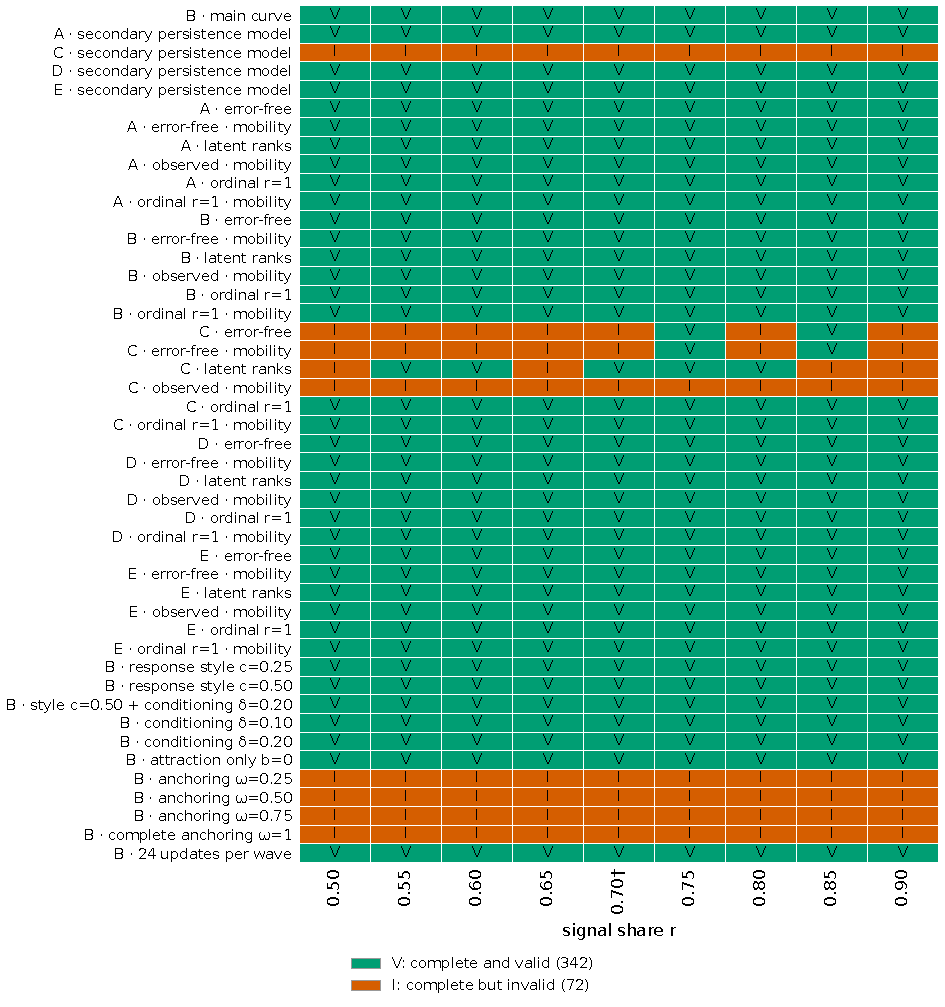
\includegraphics[width=\textwidth,height=160mm,keepaspectratio]{generated/J5_inventory_status.pdf}
\caption{Status of every unit of the prespecified inventory at the operational close, by configuration (rows) and signal share $r$. Complete and valid (V): \resultnum{v4.inv.n_valid}{342} units; Complete but invalid (I): \resultnum{v4.inv.n_invalid}{72} units; Partial at the operational close (P): \resultnum{v4.inv.n_partial}{0} units; Not started (N): \resultnum{v4.inv.n_not_started}{0} units. The legend lists only states that occur. $\dag$ $r=\resultnum{j.calibration.r}{0.70}$ was examined during calibration.}\label{fig:inventory-status}
\end{figure}



\clearpage
